\subsubsection{Palaeoceanography}


\index{Bijma, Jelle}


\paragraph{Research Team}
Jelle Bijma (Professor), Albert Benthien (postdoc), Ingrid Zondervan (postdoc), Klaus-Uwe Richter (engineer), Beate Hollmann (TA), Gernot Nehrke (PhD Student), R\'{e}gine da Rocha (PhD Student), Delphine Dissard (PhD Student)


% 150 words about research in general

In the section Marine Biogeosciences at the AWI we work on global change related issues at the level of the organism, the ecosystem or long term biogeochemical cycles. These different scales of time and space are investigated by combining experimental approaches with numerical modelling and field verification. Research topics include:
\begin{itemize}
\item Global biogeochemical cycles and specifically the role of the marine carbon cycle in global change.
\item Paleoclimatology (the glacial to interglacial transition, Holocene variability and the anthropogenic climate disturbance).
\item Stable isotope and trace element geochemistry. We are particularly keen on developing and verifying (paleo)proxies  with the aim of replacing empirical relationships by a process-based ("mechanistic") understanding (proxies are measurable descriptors (i.e. estimators) of desired but unobservable parameters and are used to reconstruct environments or climate in Earth history).
\item Marine calcification: One aspect is to determine the impact of ocean acidification on calcifying organisms, the other is to understand the mechanisms of calcification and proxie incorporation.
\end{itemize}


\paragraph{Highlights}


% 500 words about highlights in 2006

Testing prognostic climate models for future climate change critically depend on our ability to quantitatively reconstruct past climate. This basically translates to using robust proxies for paleo-temperature and -salinity in order to accurately reconstruct the thermohaline circulation (density fields). However, despite more than 50 years of paleoceanographic research, paleosalinity remains the single most important oceanographic parameter which can currently still not be quantified directly from sedimentary records. Therefore, one of the scientific highlights of this year were a couple of successful laboratory experiments towards development of such an independent salinity proxy.

Single celled marine phytoplankton (haptophyte algae, dinoflagellates and several diatom species) were cultured at different temperatures and salinities to investigate the impact of these factors on the hydrogen isotopic composition of specific compounds biosynthesized by these organisms. Two species of haptophyte algae have been analysed so far and it turned out that salinity has a substantial impact on the stable hydrogen isotopic composition of long chain alkenones ($\delta$D) and hence, that $\delta$D has a huge potential as proxy of paleosalinity \cite{Bijma1}!

In cooperation with experimental physicists from the University of M\"unster, we are getting close to determine the boron isotopic composition of single foraminiferal shells. This will allow us to estimate the the pH of deep water on the basis of benthis foraminifera, of which only few specimens are present in the cores retrieved by paleoceanographers \cite{Bijma2}.

Another highlight was the good turn-out of the field-work in Puerto Rico, where R\'{e}gine da Rocha carried out experiments on the incorporation of (trace)elements into planktonic Foraminifera. Our field- and laboratory work has been filmed and will be part of the documentary "Exploring time", produced and broadcasted by "Science Channel".


% below is a place holder for the figure, kindly send the jpeg "Jelle-fig1.jpg" with the file
% the figure caption .. is currently "xxx", please modify .. and leave the rest ..

\begin{figure}[ht]
  \begin{center}
    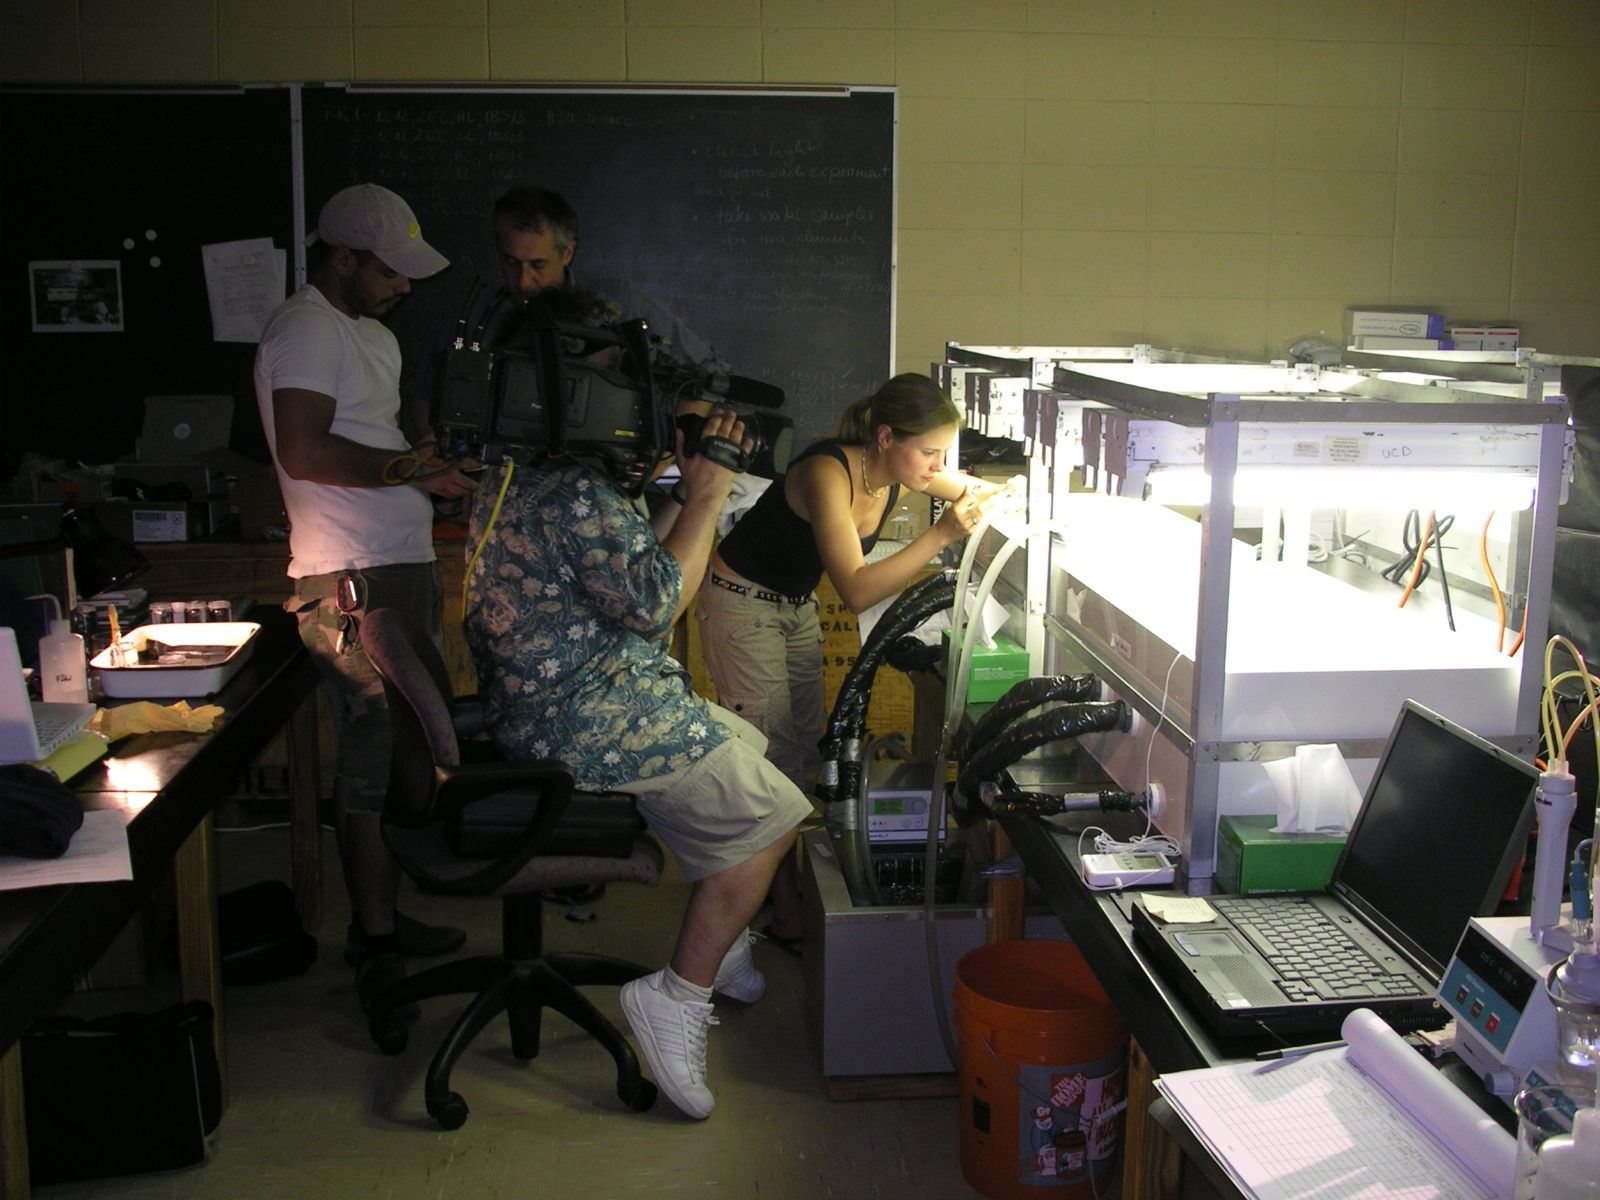
\includegraphics[width=\hsize]{Bijma/Bijma_2006_Fig.png}
    \mycaption{ %Prof. Dr. Jelle Bijma
%    \caption{
Our laboratory in Puerto Rico was turned into a filmstudio to record our contribution for the documentary `Exploring time' produced by `Science Channel'.}\label{fig:profjelle}
   \end{center}
\end{figure}

\paragraph{Organization}

% list the (research) events you have organized, if any,
% as show below space after \item and then your text ..
% if you want more, them add a new \item on a new line ..

\begin{enumerate}
\item Organisation and implementation of the annual meeting of the EU project "6C", RNIOZ, Texel, The Netherlands, 12-13 January 2006
\item Setting up a field laboratory to carry out culture experiments with planktonic Foraminifera, Magueyes Island Marine Laboratories, La Parguera, Puerto Rico, 13-26 March 2006
\item Convening several Biogeosciences sessions at the EGU general assembly, Vienna, Austria, April 2-7 April.
\item Producing part of the documentary "Exploring Time" for Science Channel, Puerto Rico, 17-24 April 2006
\item Organisation and implementation of the kick-off meeting of the ESF project "PaleoSalt", VU, Brussel, Belgium, 16-18 May 2006
\item Organisation and implementation of the final meeting of the EU project "6C", Blagnac, Bordeaux, France, 12-15 September 2006
\item Organisation and implementation of the ESF/EuroCLIMATE-EuroMinScI/ESRF Workshop entitled "Environmental Proxies: From Inorganic Precipitation to Biocrystallization", ESRF, Grenoble, France, 30-31 October 2006.
\end{enumerate}

\paragraph{Collaborations}

% The format is \item {\sl Institution} \\ Partner \\ Research Topic \ Collaboration
% Just copy and paste and change the text in "Institution"  "Partner" "Research Topic" "Collaboration"

\begin{enumerate}
\item {\sl Geology Department, University of California, Davis, USA} \\ Prof. Howard Spero
\item {\sl MARUM, University of Bremen, Germany} \\ Prof. Gerold Wefer, Prof. Dierk Hebbeln
\item {\sl Royal NIOZ (Netherlands Institute for Sea Research), Texel, The Netherlands} \\ Dr. Stefan Schouten, Dr. Geert-Jan Brummmer
\item {\sl Lab. IDES - UMR 8148, Bt 504 Geologie Universit� PARIS XI, France} \\ Prof. Jean-Pierre Cuif
\item {\sl Utrecht University, Utrecht, The Netherlands} \\ Dr. Gert-Jan Reichart, Prof. Philip van der Capellen, Dr. Mariette Wolthers
\item {\sl National Oceanography Centre, Southampton, UK} \\ Prof. Martin Palmer
\item {\sl University of Cambridge, UCAM-DES, UK} \\ Prof. Henry Elderfield
\item {\sl Laboratory of Planetary and Atmospheric Physics (LPAP) in Li\`{e}ge, Belgium} \\ Dr. Guy Munhoven
\item {\sl University of M\"unster, Germany} \\ Prof. Heinrich Arlinghaus
\item {\sl The Interuniversity Institute for Marine Science in Eilat, Israel} \\ Dr. Dan Tchernov
\item {\sl University of Hawaii, Honolulu, USA} \\ Prof. Richard Zeebe
\item {\sl Lamont-Doherty Earth Observatory, Palisades, NY, USA} \\ Dr. B\"arbel H\"onisch
\item {\sl GeoForschungsZentrum (GFZ) Potsdam, Germany} \\ Gerald Haug
\end{enumerate}


\paragraph{Grants at the Alfred Wegener Institute}
\begin{enumerate}
\item {Funded by EU} ``Carbonate Chemistry, Carbon Cycle and Climate Change ("6C": coordinator)��
\item {Funded by DFG in the framework of the bi-national collaboration with The Netherlands} ``Netherlands - Bremen - Oceanography - Science Co-Operation in Marine Research ("NEBROC": co-PI)��
\item {Funded by DFG in the framework of the bi-national collaboration with The Netherlands} ``Divalent Cations: Development and Validation of Proxy Relationships (from empirism towards a mechanistic understanding) ("Paleoprox": German-coordinator)��
\item {ESF proposal funded by DFG} ``Development, calibration and application of independent salinity proxies ("PaleoSalt": coordinator)��
\item {ESF proposal funded by DFG} ``Calcareous Biocrystals - Research on their biochemically driven crystallization mechanism and the origin of the `vital effect' ("BioCalc"; co-PI)��
\item {Funded by BMBF through collaboration with Israel} ``Reconstruction of past coral bleaching events (German coordinator).
\end{enumerate}


%Publications should be delivered as a separate file (naming convention profxxx.bib. See description by R. Helling. Please make sure that all your publications are referred to in the TeX file. This can either be in form of a \cite{profxxxkey} or as a \nocite{profxxxkey} in the end. A publication which is not reffered to on the LaTeX file doesn't produce any output in the report.

\nocite{Bijma3}
\nocite{Bijma4}
